\section{Design}

\subsection{Designkoncept}
% VICTOR do this 
\textit{[Beskriv det övergripande designkonceptet]}

Det övergripande designkonceptet baseras på [beskriv huvudidé]. Gränssnittet riktar sig till [målgrupp] och ska främst stödja [huvudsakliga uppgifter].

Designen följer principerna om [t.ex. visibility, feedback, constraints från kurslitteraturen] för att säkerställa god användbarhet.


\subsection{Iteration 1: Tidiga skisser}

I den första iterationen skapades flera olika designalternativ. Figur \ref{fig:tidiga_skisser}, \ref{fig:tidiga3} och \ref{fig:tidiga_2} visar exempel på tidiga pappersprototyper.

\begin{figure}[H]
    \centering
    \includegraphics[width=0.8\textwidth]{bilder/paper.png}
    \caption{Tidig pappersprototyper från design studio-sessionen}
    \label{fig:tidiga_skisser}
\end{figure}

\begin{figure}[H]
    \centering
    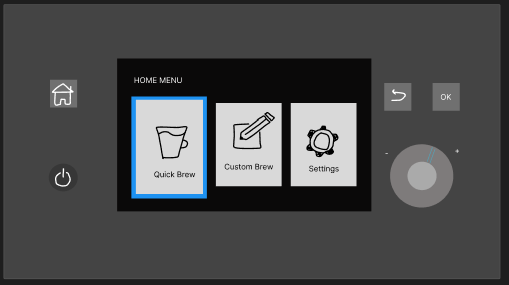
\includegraphics[width=0.8\textwidth]{bilder/victor1.png}
    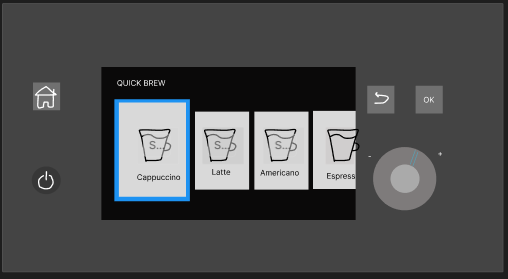
\includegraphics[width=0.8\textwidth]{bilder/victor2.png}
    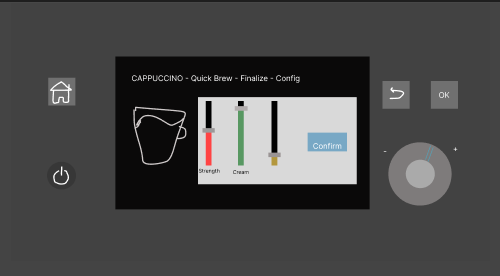
\includegraphics[width=0.8\textwidth]{bilder/victor3.png}
    \caption{Tidig prototyp från design studio-sessionen}
    \label{fig:tidiga_2}
\end{figure}

\begin{figure}[H]
    \centering
    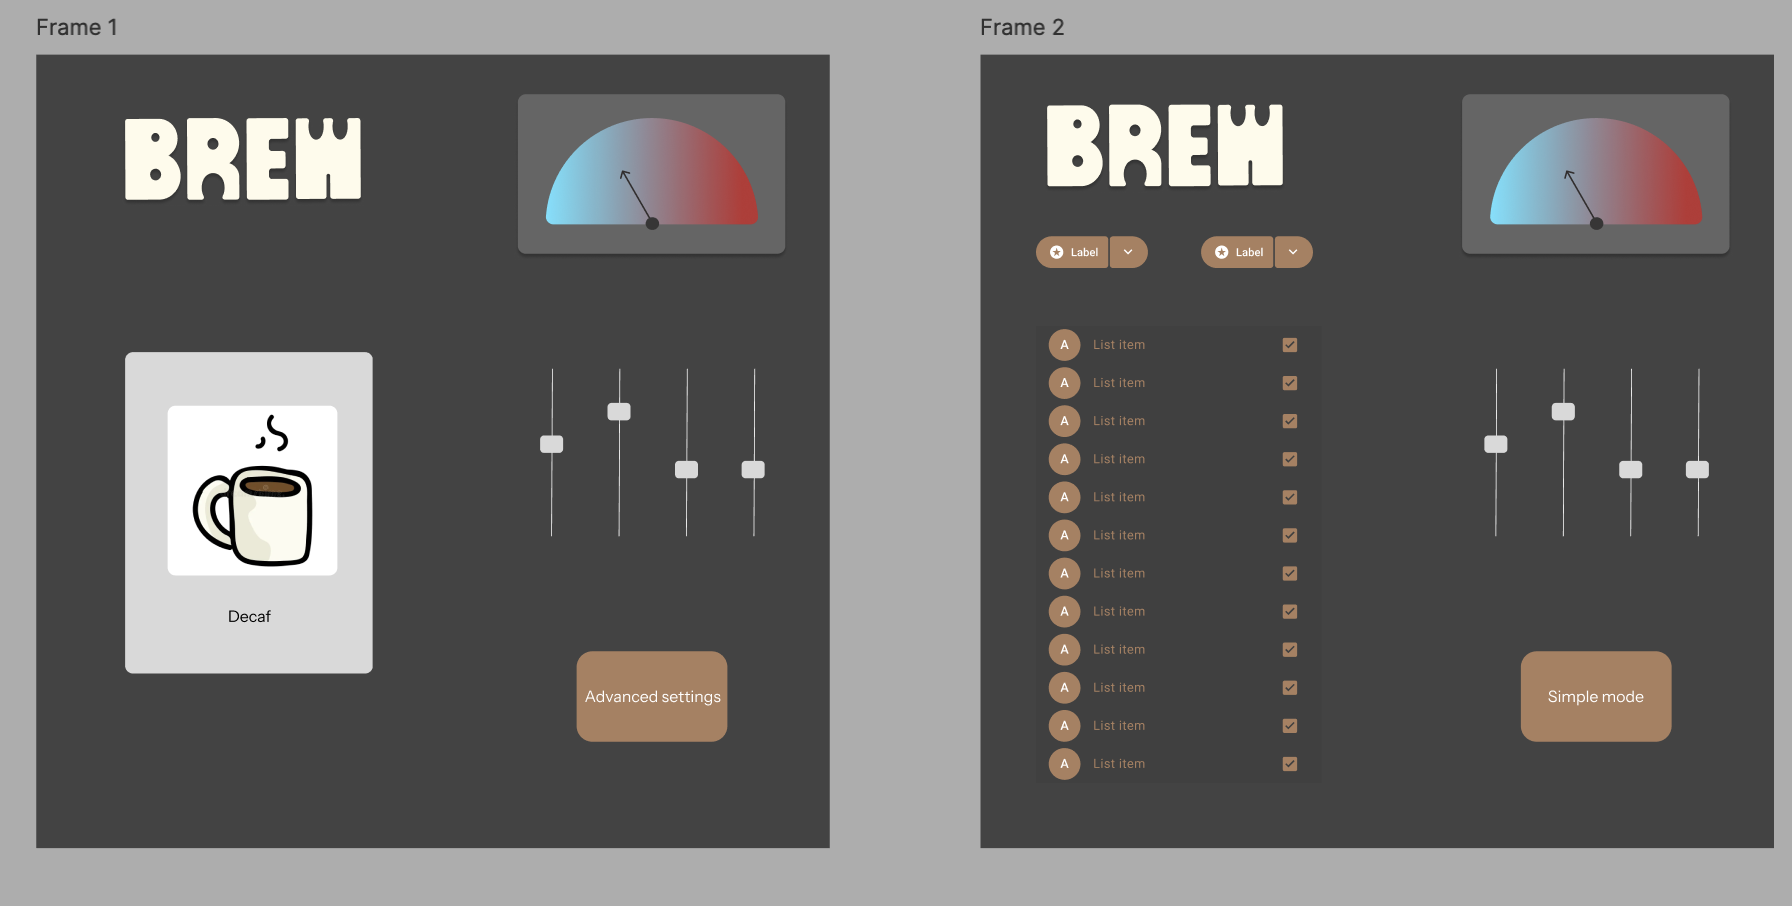
\includegraphics[width=0.8\textwidth]{bilder/sjov.png}
    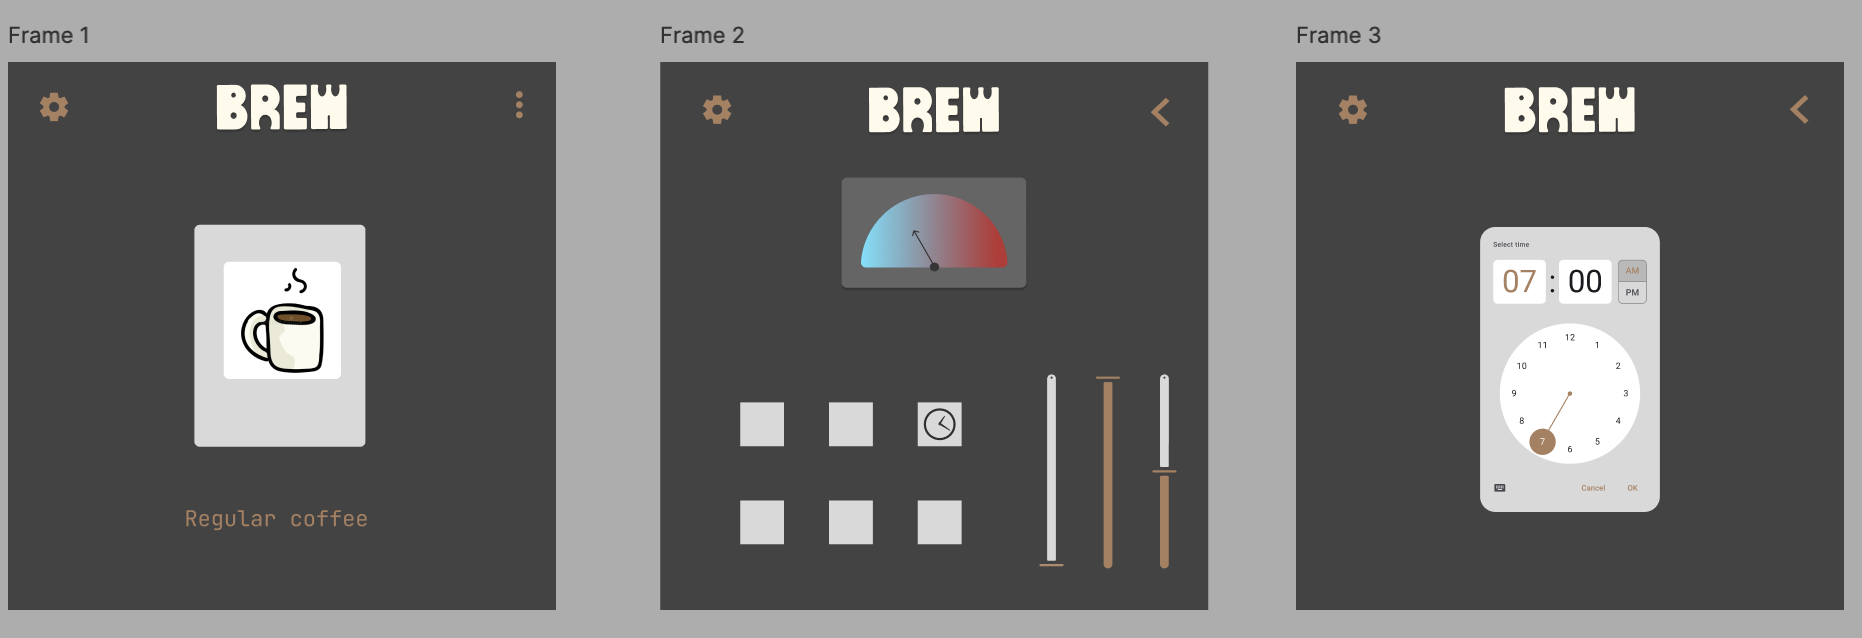
\includegraphics[width=0.8\textwidth]{bilder/sjov2.png}
    \caption{Tidig prorotyp från design studio-sessionen}
    \label{fig:tidiga3}
\end{figure}

\textbf{Designalternativ A} fokuserade på ett touchscreen-baserat gränsnit med stora kreativa grafiska representationer för information. Syftet var att skapa något tydligt som ändå hanterade avancerade inställningar väl. Detta alternativ valdes bort eftersom representationerna hade dålig överensstämmelse med mentala modellen som en typisk användare har, och var istället mer anpassat till de som redan har kunskap inom avancerat kaffe bryggning.

Exempelvis så fokuserade gränsnitet på förhålanden mellan bönor och vatten, och i termer av massa. Redan inom gruppen skappade detta förvirring, då det inte va uppenbart hur mycket man ska brygga för att få en kopp, och om det skulla göra kaffet svagare eller inte.

Det beslutades dock att id\'eerna var rimliga för ett "advanced mode" i framtida iterationer.

\textbf{Designalternativ B} erbjöd ett alternativ som använde sig av fysiska knappar och reglage. All navigation styrdes av ett hjul. Att välja alternativ var mer intuitivt, men reglagen gjorde det svårare att använda avancerade inställningarna, och var inte praktiskt för att namnge profiler. 

\textbf{Designalternativ C} fokuserade på touch, och tillämpade en “plattare” design. Fler alternativ, inställningar, och funktioner kunde visas, och färre steg var obligatoriska för att brygga kaffe. Därför valdes det att basera första digitala prototypen på detta alternativ.
\subsection{Iteration 2: Första digitala prototyp}


Baserat på feedback från lo-fi-testerna utvecklades den första digitala prototypen.  Detta gjordes genom en bedömning för varenda design mål för alla koncept samt vilka design constraints de hade. Koncepten för avancerat läge togs från alternativ A, preset design togs från alternativ B och C, och schemaläggning inspireras av fig alternativ C. Det skapades först en lofi prototyp, och utefter den skapades en interaktiv prototyp med javascript. Huvudsakliga vyer inkluderar: startsidan, sidmenyn, “manage profiles”, “schedule coffee” och "create profile".

\begin{figure}{H}
    \begin{center}
        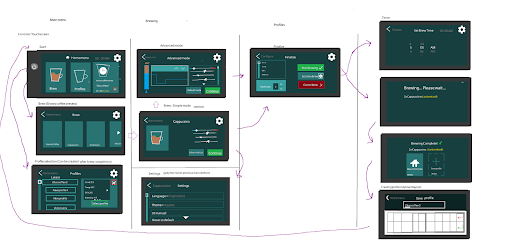
\includegraphics[width=0.95\textwidth]{bilder/victorM.png}
    \end{center}
    \caption{Merged koncept av alla gruppmedlemmars första koncept.}
    \label{fig:mergedV}
\end{figure}

\subsubsection{Startsida}

Startsidan designades för att tillåta användaren att brygga sin kaffe så fort som möjligt. Genom att flytta alla diagram och inställningar till andra delar av gränssnittet blir det tydligt vilka alternativ man har. Om man bara vill ha kaffe, då trycks det på quick brew. Om man vill leka med inställningar eller presets så trycker man på plus. Mellan lofi och hifi prototyperna så flyttades även diagrammen till “edit profile” skärmen. Tillsammans bidrar detta till teoretisk bättre visibility, samt bättre sammanhang mellan användarens mentala modell och gränssnitt. Exempelvis är det tydligt att “quick brew” inte är en preset, och kan inte förändras. 

Inom denna prototyp så var affordance i huvudfokus pågrund av idén för en kaffemaskin så skulle touchskärm integreras pågrund av constraints för fanns för fysiska knappar, men dessutom så kan det vara så att skärmen inte är tillräckligt stor, så pga visibility så var därför affordance i huvudfokus. Tydligaste exemplaret av affordance är när man ska klicka "Brew" där menyn visas i block där den längst till vänster visade att man kunde "swipea" höger. Risken med detta var dock memorability ifall man kommer ihåg att ett visst preset fanns längst till höger om man ville bara brygga en enkel kopp macchiato t.ex. Alla knappar inom menyn ska dessutom vara lätt igenkännbara med att de går att trycka på, så de mesta knappar ska ha en rektangulär form med runda kanter som påminnelse att de går att trycka på för att uppfylla design constraint affordance.

\begin{figure}[H]
    \centering
    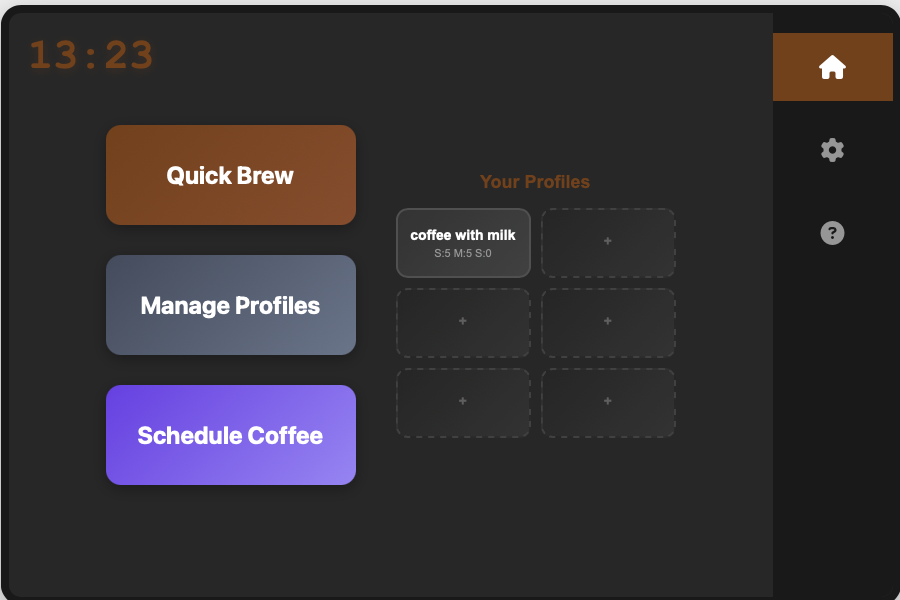
\includegraphics[width=0.6\textwidth]{bilder/start.png}
    \caption{Första versionen av startsidan}
    \label{fig:startsida_v1}
\end{figure}

Huvudelementen är:
\begin{itemize}
    \item \textbf{Quick Brew}: Placerad i toppen av menyn till vänster, för att göra det tydligt att den inte är en preset, samt är den stor så att det blir en av de första sakerna som märks av användaren. Detta minskar chansen att en användare inte lyckas brygga kaffe alls.     

    \item \textbf{Preset area}: Placerat till höger, och någorlunda mindre än menyn till vänster. Strukturen görs så att mindre scrollning behövs jämfört med tidiga prototyper, och skapar en tydlig skillnad mellan det man kan ändra, och det som är permanent. 
\end{itemize}

\subsubsection{Manage Profiles}

Sidan designades för att tillåta användaren att redigera eller ta bort profiler. Elementen ordnas i en enkel lista för att göra det så tydligt som möjligt för användaren att de redigerar och inte brygger. Valet att ha en separat skärm för detta gjordes för att förenkla startsidan så mycket som möjligt.
\begin{figure}[H]
    \centering
    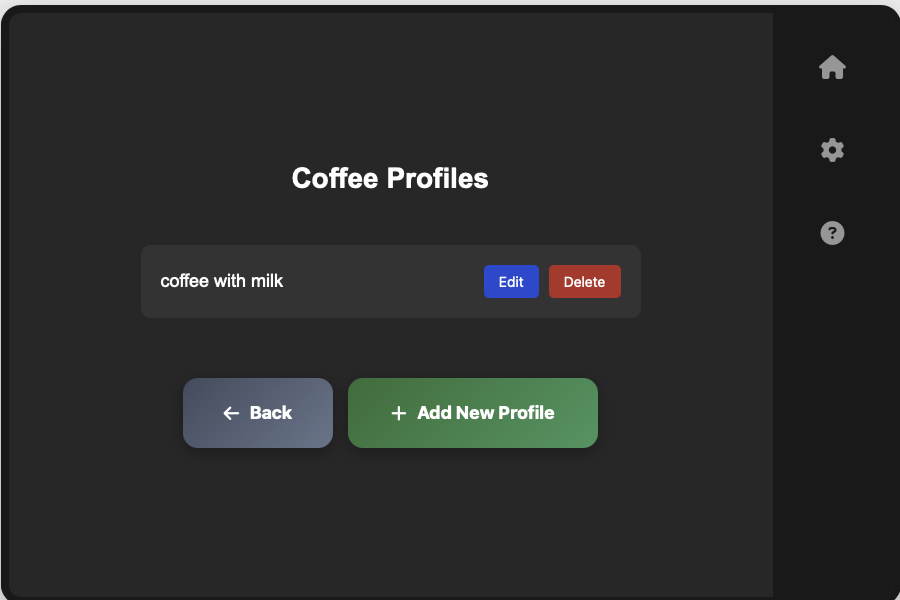
\includegraphics[width=0.6\textwidth]{bilder/manage.png}
    \caption{Första versionen av "manage profles" sidan}
    \label{fig:manage_v1}
\end{figure}

\subsubsection{Schedule Coffee}

Sidan designades för att tillåta användaren att schemalägga en bryggning. Layouten följer samma format som “Manag Profiles"-sidan. Genom att göra det konsekvent förstår användaren åter att listan finns för att redigera, och att knapparna är permanenta. 
\begin{figure}[H]
    \centering
    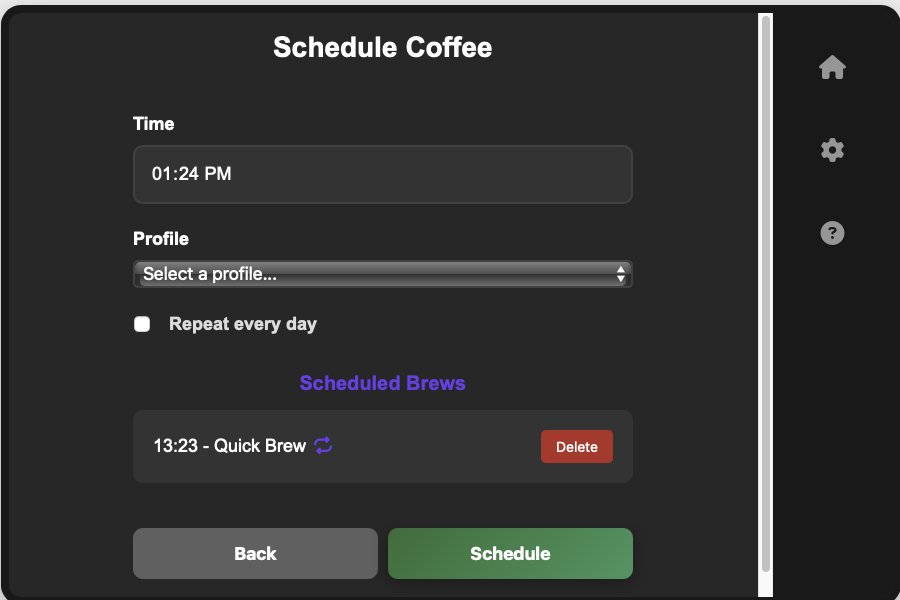
\includegraphics[width=0.6\textwidth]{bilder/schedule.png}
    \caption{Första versionen av "schedule coffee" sidan}
    \label{fig:schedule_v1}
\end{figure}

Huvudelementen är:
\begin{itemize}
    \item \textbf{Scheduled Brews}: Följer samma principer som "manage profiles".
    \item \textbf{Select a profile}: Använder sig av en "pop down menu" för att minska hur mycket information behövs bearbeta direkt då en användare får upp skärmen. 
    \item \textbf{Time}: Placerat längst upp, eftersom det är det användaren tänker på först när de vill schemalägga något. 
\end{itemize}


% ================ Create Profile ==================
\subsubsection{Create Profile}
Det bestämdes tidigt att “Create pofile” sidan var väldigt viktig. Den behöver vara enkel nog för att inte skrämma bort användare som inte har stor kompetens inom kaffe-bryggning eller teknik, men också vara intuitiv, effektiv, och kul att använda för de som har dem kompetenserna. 

\begin{figure}[H]
    \centering
    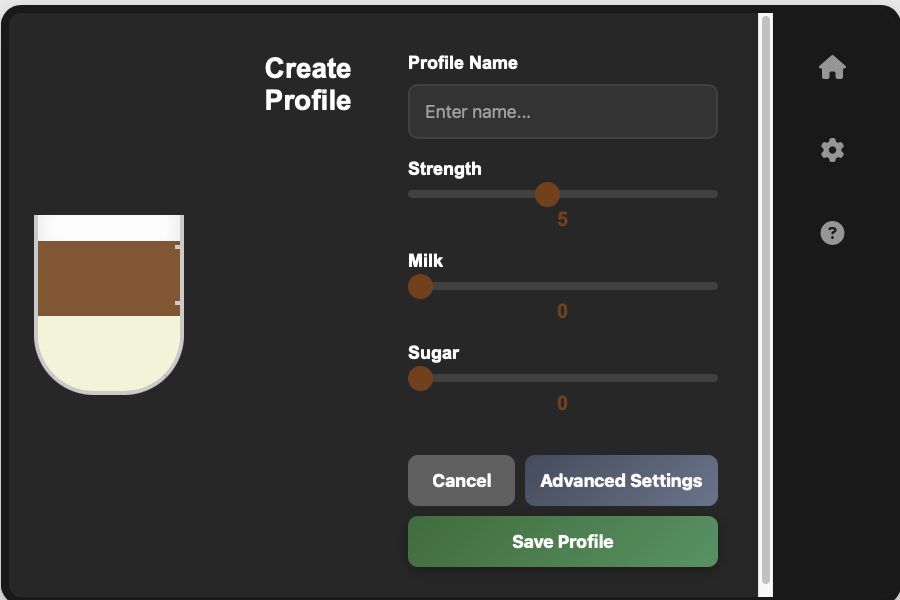
\includegraphics[width=0.6\textwidth]{bilder/brew.png}
    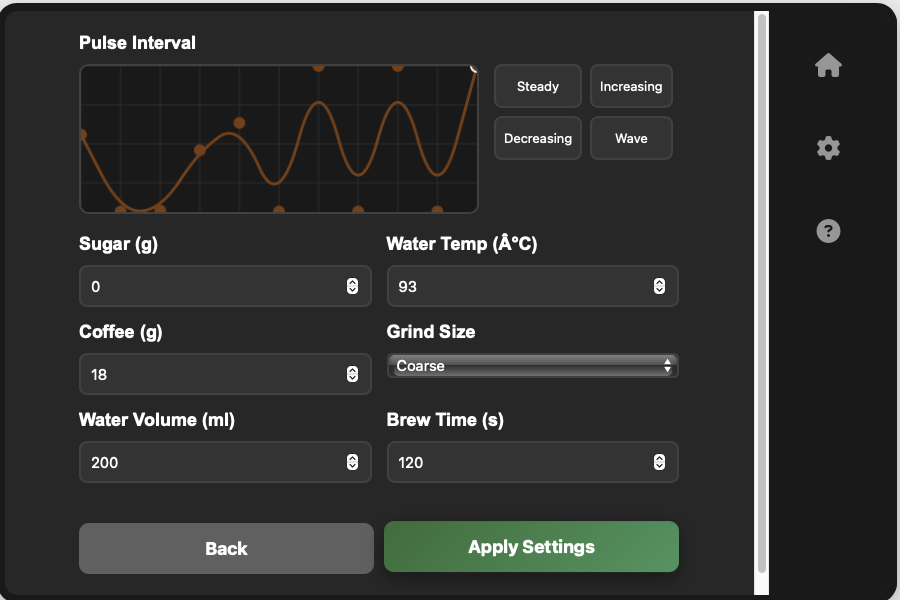
\includegraphics[width=0.6\textwidth]{bilder/advancedshit.png}
    \caption{Första versionen av "create profiles" sidan}
    \label{fig:create_v1}
\end{figure}
\textbf{Utility}: Prototypen utnyttjar verktyg för att kunna utföra kaffebryggning på både ett enkelt och avancerat sätt, men på en funktionalitet så att användaren får specificera hur i detalj de vill gå. Användaren borde kunna ändra enkla saker som förekommer oftast vid kaffebryggning, såsom mjölk, styrka och socker, då det är en väldigt vanlig smaksak. När det dock kommer de som vill experimentera lite mer med sitt kaffe så finns därför ett avanced mode för att kunna vara så precis som möjligt med sin kaffebryggning. Där kan användaren konfigurera pulsintervall för kaffebryggning, andel socker i gram, temperaturen på kaffet, andel kaffe i gram, texturen på kaffet, andel vatten som används och hur länge det ska bryggas i.

\textbf{Effectiveness}: Eftersom att den ordinära användaren inte vill trycka in andel socker eller vattentemperatur så borde de inte finnas inom defaultkonfigurationen pågrund av att en kaffemaskin främst ska göra kaffe på ett snabbt och effektivt sätt, så om man behöver knappa in mer saker i en defaultkonfiguration för kaffe så kan det göra användaren överväldigad med andelen funktioner för att bara brygga kaffet. Därför finns advanced mode som en separat meny för de som är medvetna om att de kan lite mer om kaffe men samtidigt ska det inte låsa ut användare för att pröva och experimenta med sitt kaffe om de vill.

\textbf{Efficiency}: Profilmenyn är designat så att vid defaultkonfigurationen av att skapa en profil så är det simplicietet som är i prioritet, så att användaren kan brygga kaffe så snabbt som möjligt med ett enkelt utseende på skärmen. Om användaren vill gå in i detalj så finns advanced mode för det alternativet. Det är medvetet att det kommer ta mer tid, men samtidigt så går det ändå att göra menyn tilräckligt enkel för att inte skrämma bort användare som vill testa sig fram genom menyerna. Detta görs t.ex genom presets för pulsintervallet.

\textbf{Learnability}: Med ett enkelt gränssnitt så ska det vara enkelt att göra sitt kaffe men inte "skrämma" användare för att experimentera med advanced modes funktioner. Därför behövde vara enkel att lära sig med att inte ha för många funktioner med samtidigt tillfredsställa de som vill konfigurera sitt kaffe.

Advanced menyn förenklades med att tydliggöra pulsintervallet, samt ge användaren presets att välja från, för att hen ska kunna få en känsla för gränssnittet.


% ================  Side menu ==================
\subsubsection{Sidmenyn}
Sidmenyn designades för att ge snabb åtkomst till viktiga funktioner som kan behövas oavsett var man är i gränssnittet.  

Huvudelementen är:
\begin{itemize}
    \item \textbf{Hem Knappen}: Placerad längst upp för att skapa ett sätt för användaren att alltid kunna komma tillbaka till startsidan. Detta hjälper mycket med att minska antalet fel som inte går att åtgärda. 
    \item \textbf{Inställningar och hjälp}: Synligt placerad eftersom användaren ska alltid kunna få hjälp. Kravet för användaren att behöva komma ihåg saker minskas.
\end{itemize}



% ========================= CONTINUING HERE ======================

\subsection{Iteration 3}

Efter användbarhetstester i iteration 2 identifierades flera problem (se avsnitt \ref{sec:resultat_test}). Följande ändringar gjordes:


\begin{figure}[H]
    \centering
    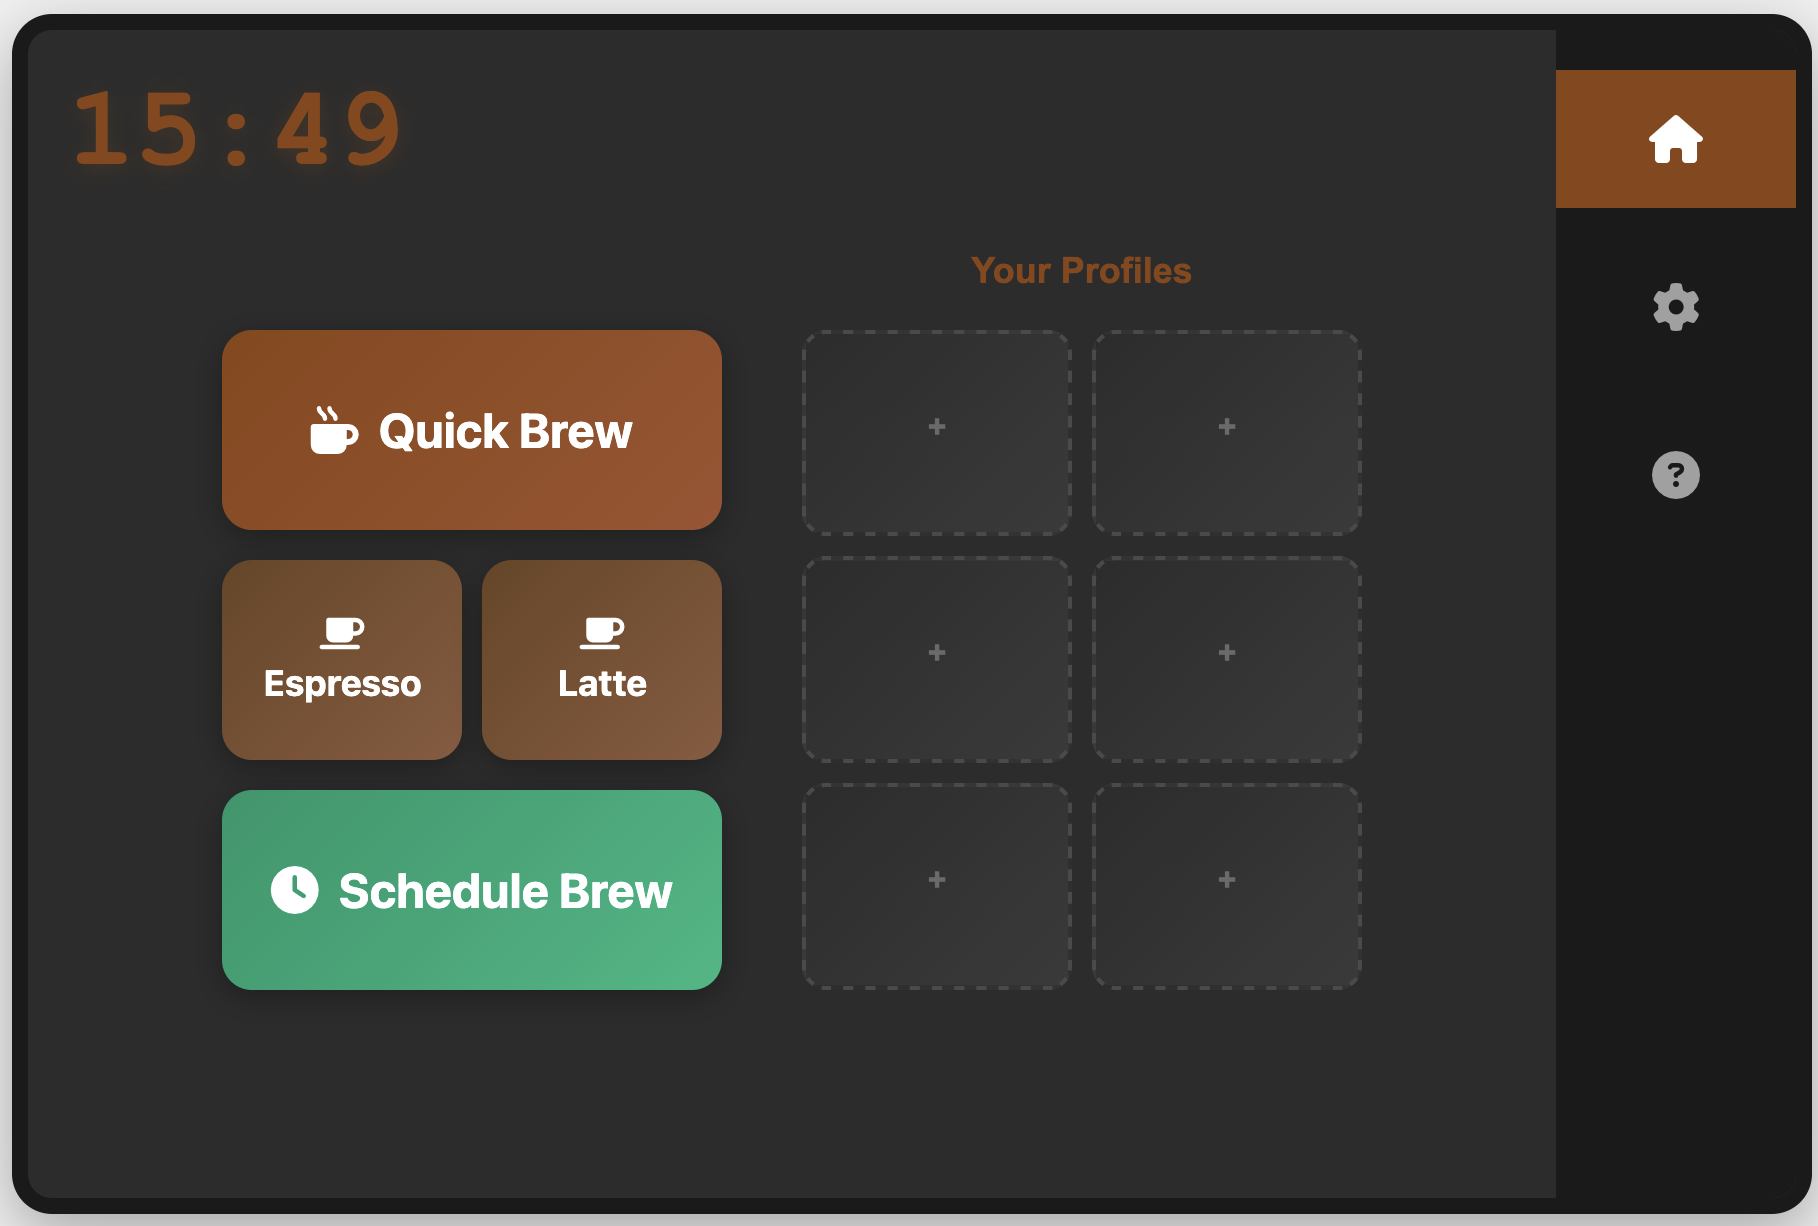
\includegraphics[width=0.6\textwidth]{bilder/3problem1-25.png}
    \caption{ förändringar som gjorts för att lösa problem 1, 2 och 5}
    \label{fig:forbattring1}
\end{figure}

\textbf{Problem 1:} Användare hade svårt att identifiera vad knappar gjorde direkt, och tyckte att det var krävande att behöva läsa så mycket text.  

\textbf{Lösning:} Fler ikoner lags till som anseddes förbättra tydligheten av knapparna samt följer det Nielsens (citation) design heurestic “Recognition over recall”. 

\textbf{Problem 2} Flera användare tyckte att det borde finnas färdiga profiler 

 \textbf{Lösning:} Färdiga profiler skapades. De går att använda profilerna som avgångspunkter för att skapa eget recept, detta tycktes göra processen enklare för de som inte har mycket erfarenhet inom kaffe.  

 \textbf{Problem 3} Vi fick feedback att färgerna var ibland inte konsekventa, och att de var ibland otydliga.  

\begin{figure}[H]
    \centering
    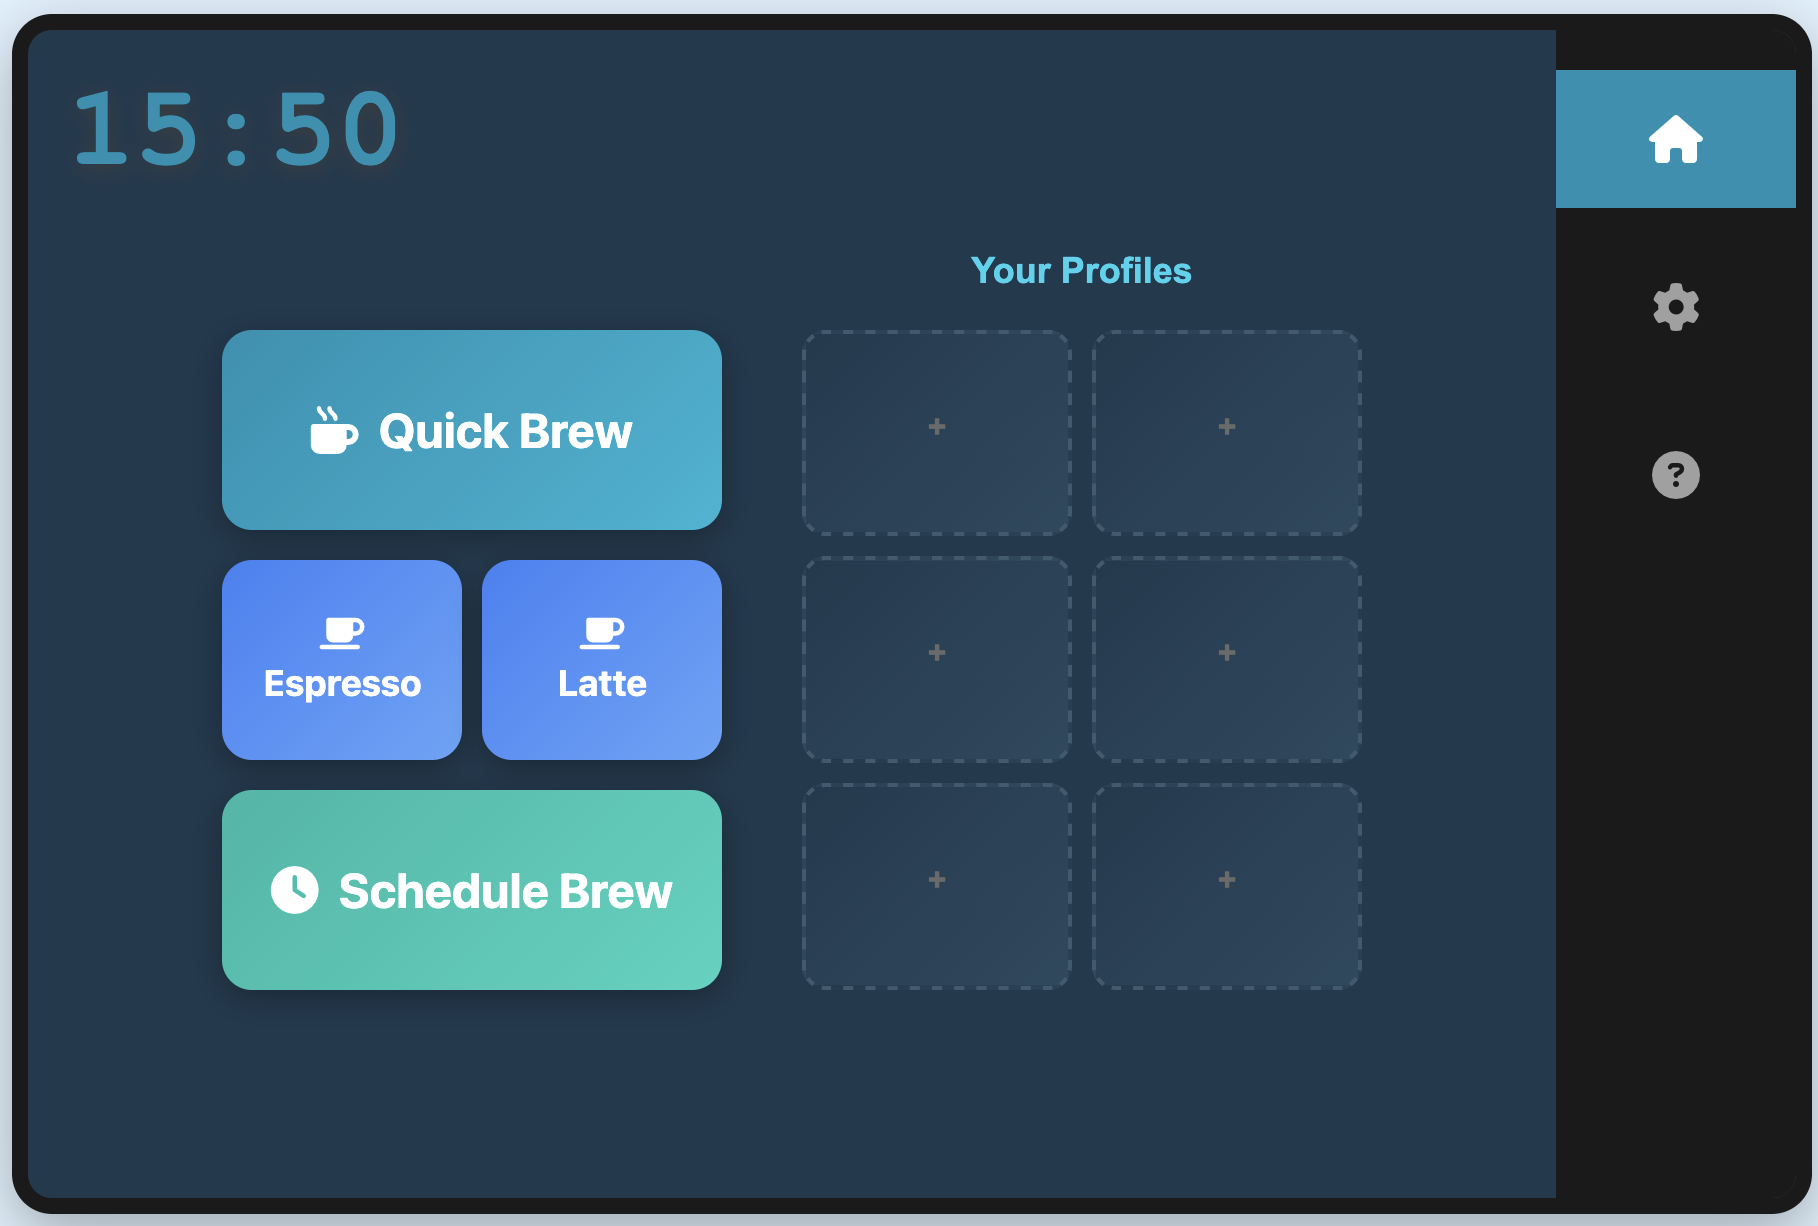
\includegraphics[width=0.6\textwidth]{bilder/3problem2.png}
    \caption{ förändringar som gjorts för att lösa problem 3}
    \label{fig:2forbattring2}
\end{figure}
\textbf{Lösning:}  flera påpekade detta problem, men hade inte specifika krav eller exempel. På grund av detta samt att flera andra ville ha valbara färgtema, så var det naturligt att implementera några färgteman.   

\textbf{Problem 4} Gränssnittet för att schemalägga bryggning hade fåt lite kritik över des icke intuitive design. 

\begin{figure}[H]
    \centering
    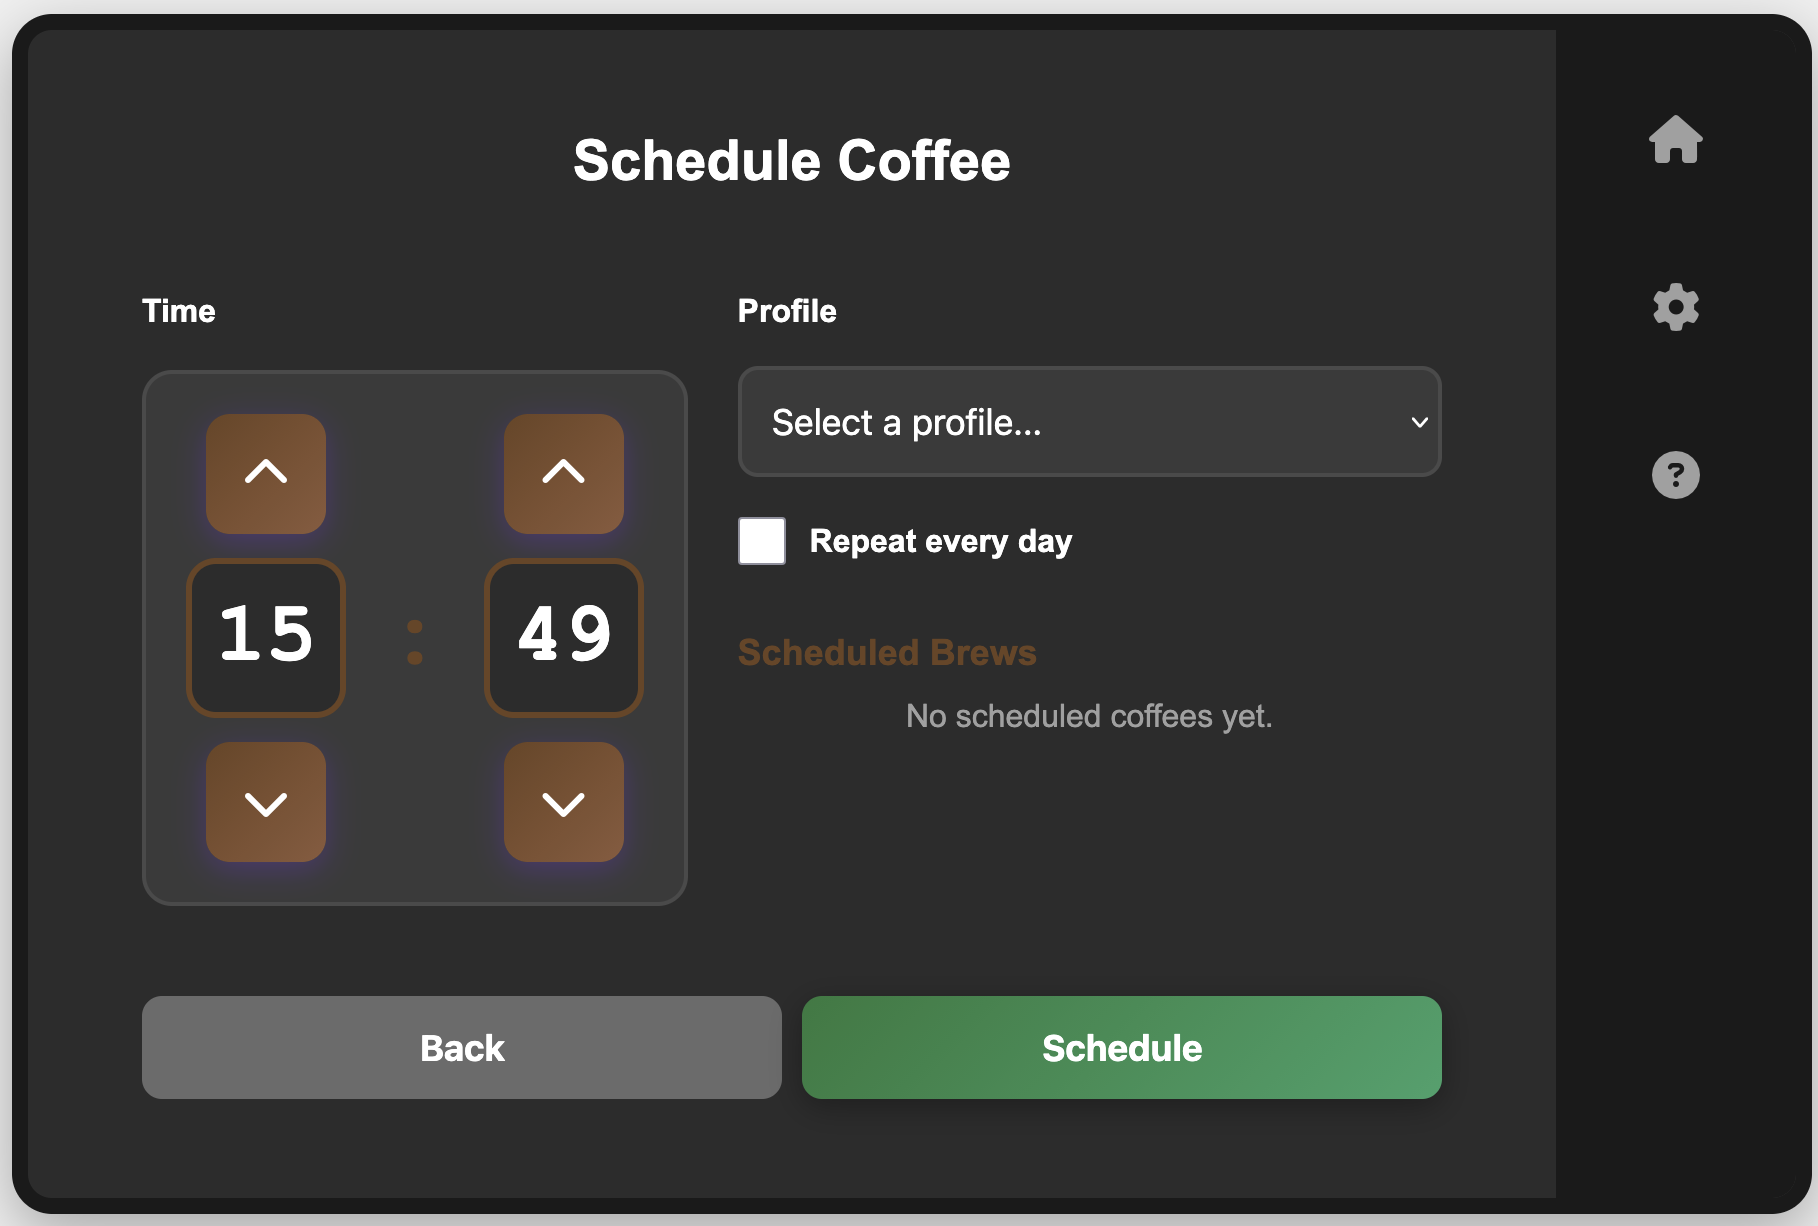
\includegraphics[width=0.6\textwidth]{bilder/3problem4.png}
    \caption{ förändringar som gjorts för att lösa problem 4}
    \label{fig:forbattring3}
\end{figure}
\textbf{Lösning} Det gjordes om så att knappar användes för att välja tid. Detta anseddes vara lättare än att skriva in tiden med ett touch tangentbord på skärmen  

 \textbf{Problem 5} “Profile manager” sidan förvirrade visa användare.  

\textbf{Lösning:} Detta var ganska logiskt, eftersom det går att skapa profiler från startsidan så borde det också gå att redigera dem där. Därför lags det till en “edit” knapp  på var profil i startsidan, och delete knappen flytades in i “edit profile” vyn.  Därefter så togs bort “Profile manager” sidan.  






\subsection{Iteration 4}

Efter användbarhetstester i iteration 3 identifierades flera problem (se avsnitt \ref{sec:resultat_test}). Följande ändringar gjordes:

\textbf{Problem 1:} Kontrasten gjorde viss text otydlig eller svår att läsa.  

  

\textbf{Lösning:} Det lags till en lysande effekt till text där det anseddes vara ett problem med kontrast. Samt lags det till en “blinking” effekt till visa textfält för att förtyda att de var obligitoriska.  

  
\begin{figure}[H]
    \centering
    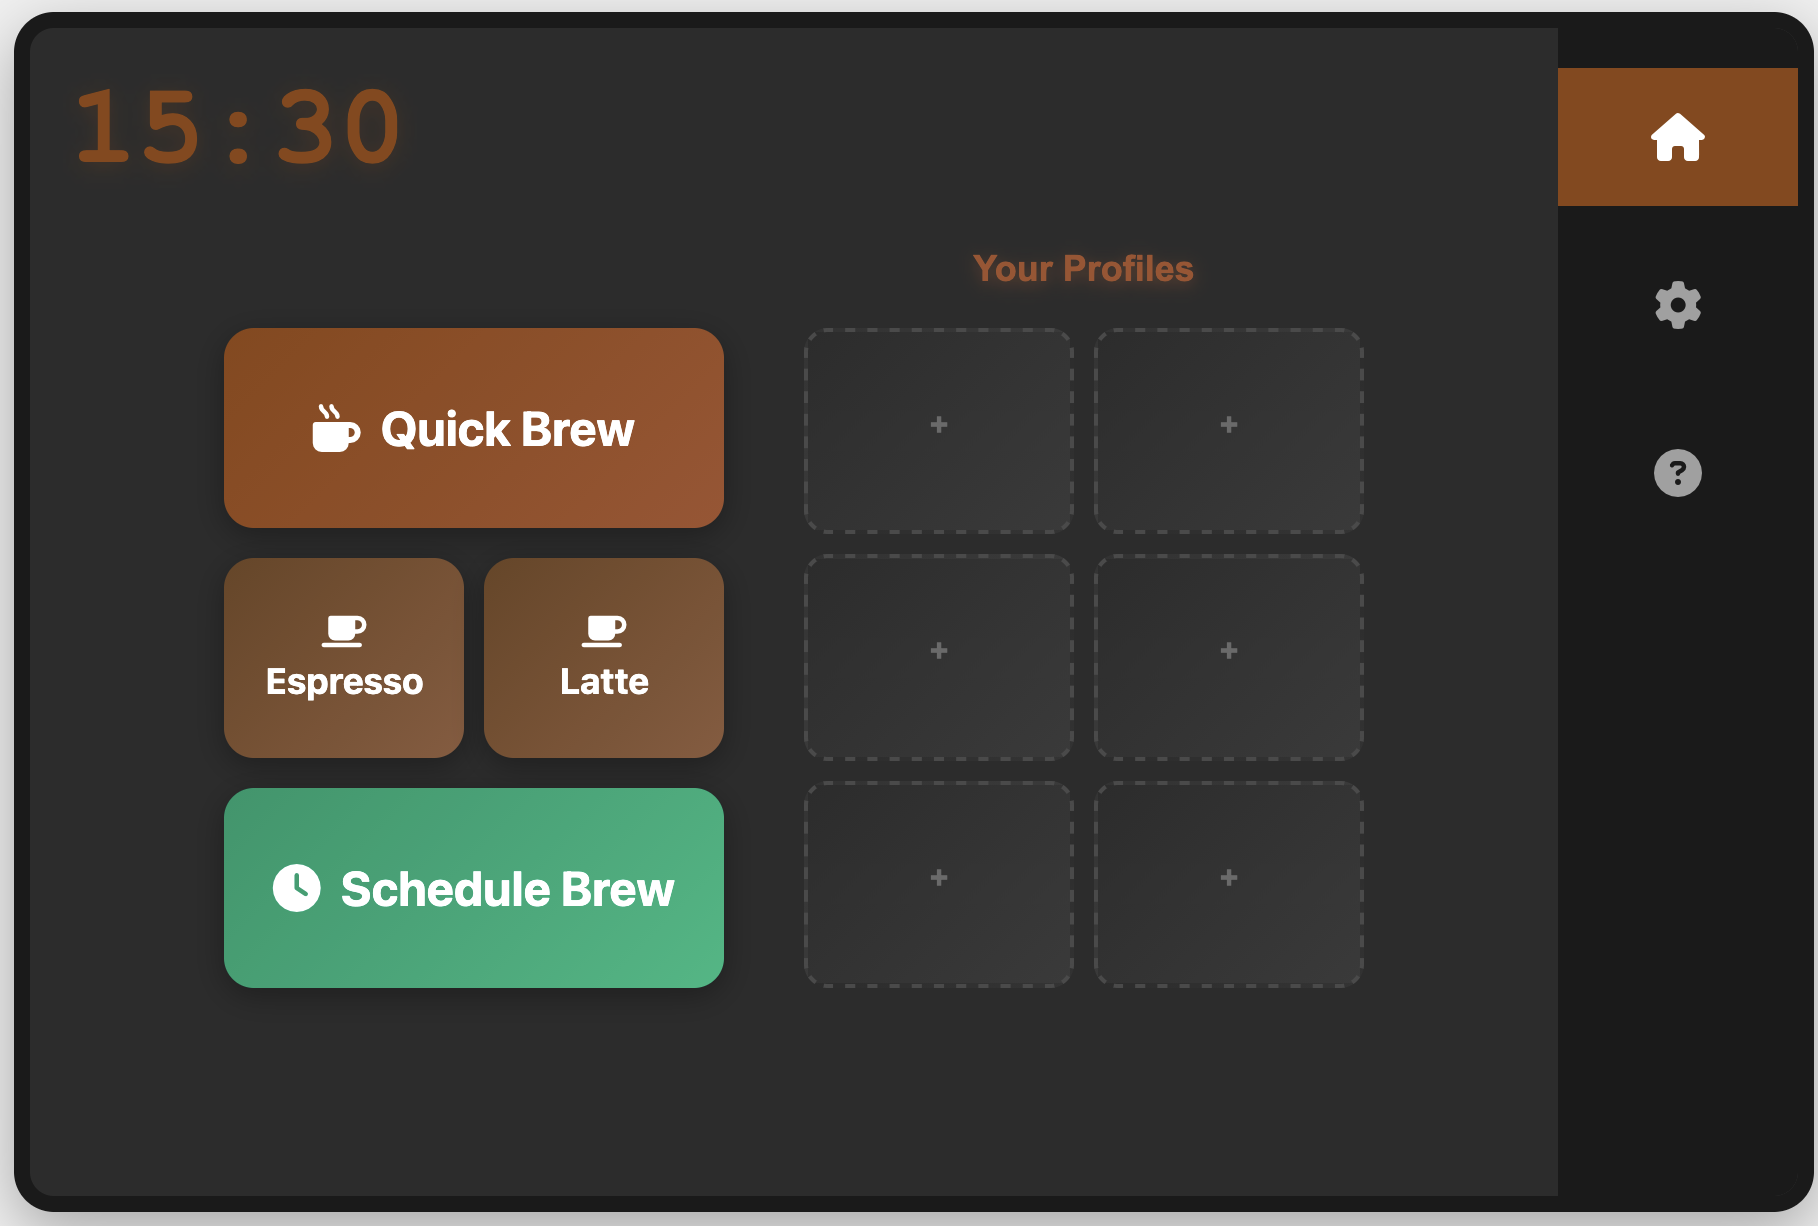
\includegraphics[width=0.6\textwidth]{bilder/3problem1.png}
    \caption{ förändringar som gjorts för att lösa problem 1}
    \label{fig:forbattring4}
\end{figure}

\textbf{Problem 2} “Confirm” menyer var ej konsekventa och ibland saknades det en “cancel knapp” 

  

\textbf{Lösning:} En “cancel” knapp lags till i varje “confirm” meny, samt  
standardiserades de över hela gränssnittet.  

\textbf{Lösning:}  

Detta var ganska logiskt, eftersom det går att skapa profiler från startsidan så borde det också gå att redigera dem där. Därför lags det till en “edit” knapp  på var profil i startsidan, och delete knappen flytades in i “edit profile” vyn.  Därefter så togs bort “Profile manager” sidan.  


\begin{figure}[H]
    \centering
    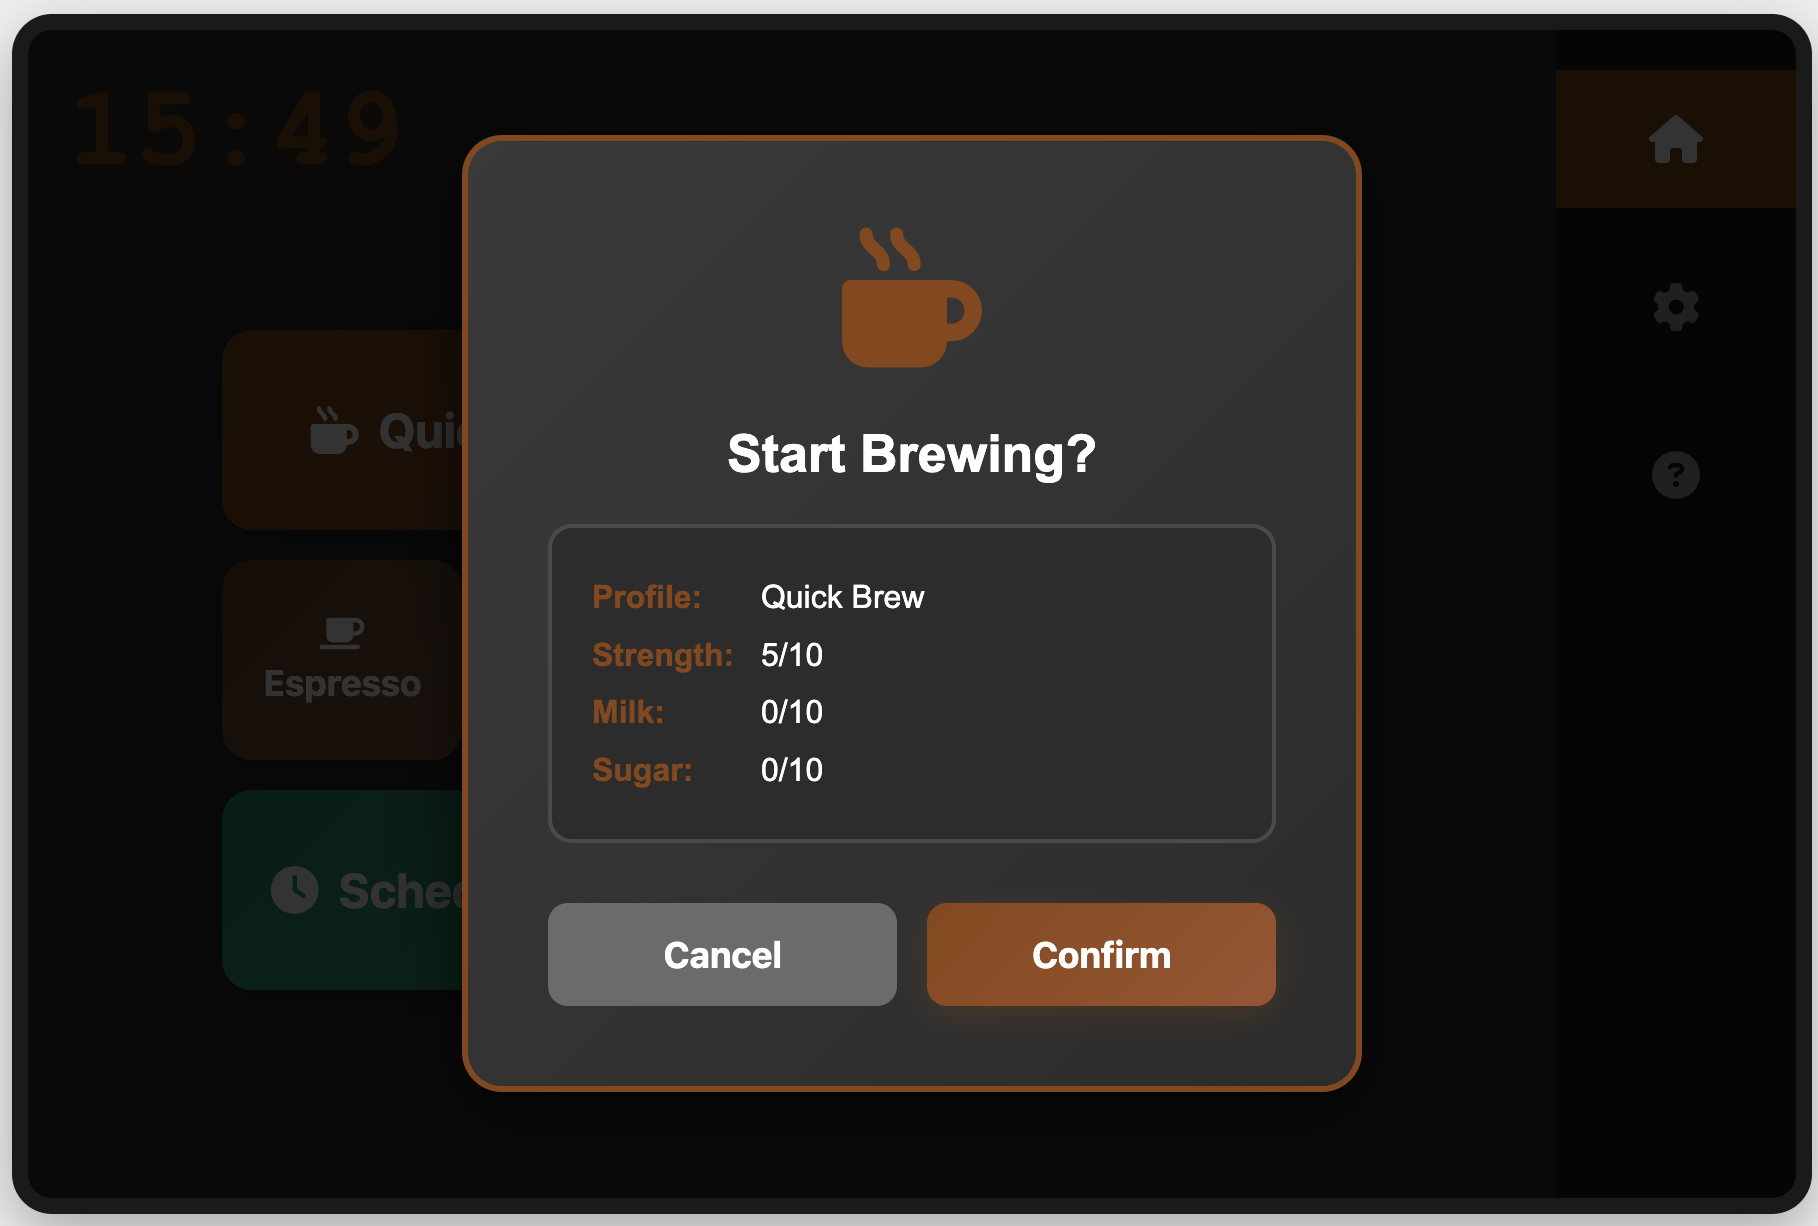
\includegraphics[width=0.6\textwidth]{bilder/4problem2.png}
    \caption{ förändringar som gjorts för att lösa problem 2}
    \label{fig:forbattring5}
\end{figure}


\subsection{Slutgiltig design}

\textit{[Presentera den slutgiltiga designen]}

Den slutgiltiga designen är resultat av [antal] iterationer och integrerar feedback från [antal] användare. Fullständiga vyer finns i Bilaga C.

Huvudsakliga designprinciper som tillämpats:
\begin{itemize}
    \item \textbf{Konsistens}: Alla vyer följer samma layoutmönster...
    \item \textbf{Feedback}: Användaren får tydlig återkoppling när...
    \item \textbf{Affordance}: Interaktiva element signalerar tydligt...
\end{itemize}




\subsection{Designbeslut och motiveringar}

\textit{[Sammanfatta viktiga designbeslut]}

\begin{table}[h]
\centering
\begin{tabular}{|p{4cm}|p{5cm}|p{4cm}|}
\hline
\textbf{Designbeslut} & \textbf{Motivering} & \textbf{Teoretisk grund} \\
\hline
Navigation i top bar & Användarna förväntar sig... & Mental modeller \cite{sharp2019} \\
\hline
Färgschema: ... & Tillgänglighet och kontrast & WCAG-riktlinjer \\
\hline
... & ... & ... \\
\hline
\end{tabular}
\caption{Sammanställning av huvudsakliga designbeslut}
\end{table}
